%% 02-covariates-short.tex — Sant'Anna Workshop Pisa: Covariates in DiD (shortened)
%% Scott Cunningham, Sant'Anna Workshop on Causal Inference, Pisa
%% Principle: one idea per slide. No walls of text.

\documentclass[aspectratio=169,11pt]{beamer}
\usepackage{remix}
\usepackage{madrid_theme}

\usepackage{tikz}
\usetikzlibrary{positioning,arrows.meta,calc,shapes.geometric,fit,backgrounds}
\usepackage{listings}
\usepackage{xcolor}
\usepackage{booktabs}
\usepackage{colortbl}
\usepackage{amsmath}

\lstset{
  basicstyle=\ttfamily\footnotesize,
  keywordstyle=\color{accentdark}\bfseries,
  commentstyle=\color{warmgray}\itshape,
  stringstyle=\color{ocean},
  backgroundcolor=\color{lightbg},
  frame=single, framesep=4pt,
  rulecolor=\color{warmgray!40},
  columns=fullflexible,
  showstringspaces=false,
  breaklines=true,
  numbers=none,
  xleftmargin=0.4em, xrightmargin=0.4em,
}

\newcommand{\emphbox}[1]{%
  \begin{beamercolorbox}[rounded=true,sep=7pt,wd=\linewidth]{block body}%
    \small\color{slate} #1%
  \end{beamercolorbox}}

\begin{document}

%% ---------- TITLE ----------
\codechellatitle
  {Covariates in DiD}
  {OLS specs, IPW, OR, DR}
  {Scott Cunningham \textperiodcentered\ Baylor University}
  {Sant'Anna Workshop on Causal Inference \textperiodcentered\ Pisa}

%% ---------- RECAP ----------
\begin{frame}{Yesterday: three problems with additive covariates}
\vspace{0.4em}
\begin{enumerate}\setlength\itemsep{0.5em}
  \item \textbf{Heterogeneous treatment effects in $X$} \hfill \highlight{Fix: interact $D \times X$}
  \item \textbf{Imbalance + differential trends} \hfill \highlight{Fix: interact $\text{Post} \times X$}\\
        {\small\color{warmgray}(including time-invariant $X$ --- but \textbf{never} post-treatment $X$)}
  \item \textbf{Time-invariant $X$ absorbed by unit FE} \hfill \highlight{Drops out entirely}
\end{enumerate}
\vspace{0.5em}
\begin{center}\color{warmgray}\small
Today: a brisk review of OR, IPW, and DR; simulation; LaLonde application.
\end{center}
\end{frame}

%% ---------- SCHEDULE ----------
\begin{frame}{Thursday: we are behind, so we accelerate}
\vspace{0.5em}
\begin{enumerate}\setlength\itemsep{0.5em}
  \item \highlight{Covariates (now):} OR, IPW, DR --- and the LaLonde lab
  \item \highlight{Continuous DiD:} TWFE decomposition, causal parameters, estimation + exercise
  \item \highlight{Staggered adoption:} TWFE problems, Callaway--Sant'Anna
  \item \highlight{Claude Code:} live demo, zero-shot pipeline, verification
\end{enumerate}
\vspace{0.5em}
\begin{center}\color{warmgray}\small
Synthetic control: probably not today.
\end{center}
\end{frame}

%% ====================================================================
%% PART 1 — OLS SPECIFICATIONS
%% ====================================================================

\begin{frame}{The standard TWFE with additive $X$}
\vspace{1.2em}
\begin{center}
\large
$Y_{it} \;=\; \alpha_i + \lambda_t
      + \delta\,(D_i \times \mathrm{Post}_t)
      + \boldsymbol{\beta}\,X_i
      + \varepsilon_{it}$
\end{center}
\vspace{1.0em}
\begin{center}
Two hidden assumptions:
\begin{enumerate}
  \item Returns to $X$ are \textbf{constant over time}
  \item Treatment effect is \textbf{the same for all $X$}
\end{enumerate}
\end{center}
\end{frame}

%% ----------
\begin{frame}{Worry 1: $\beta$ changes at the policy break}
\vspace{1.0em}
\begin{center}
\large
$Y_{it} \;=\; \alpha_i + \lambda_t
      + \delta\,(D_i \times \mathrm{Post}_t)
      + \boldsymbol{\beta}\,X_i
      + {\color{accent}\boldsymbol{\gamma}\,(\mathrm{Post}_t \times X_i)}
      + \varepsilon_{it}$
\end{center}
\vspace{0.8em}
\begin{center}
\color{warmgray}\small
$\boldsymbol{\gamma}$ absorbs any shift in returns to $X$ between pre and post.
\end{center}
\end{frame}

%% ----------
\begin{frame}{Worry 2: treatment effect varies with $X$}
\vspace{1.0em}
\begin{center}
\large
$Y_{it} \;=\; \alpha_i + \lambda_t
      + \delta_0\,(D_i \times \mathrm{Post}_t)
      + {\color{accent}\boldsymbol{\tau}\,(D_i \times \mathrm{Post}_t \times X_i)}
      + \boldsymbol{\beta}\,X_i
      + \varepsilon_{it}$
\end{center}
\vspace{0.8em}
\begin{center}
\color{warmgray}\small
ATT $= \frac{1}{n_T}\displaystyle\sum_{D_i=1} \bigl(\hat\delta_0 + \hat{\boldsymbol{\tau}}\,X_i\bigr)$
\end{center}
\end{frame}

%% ----------
\begin{frame}{Both worries: the fully saturated spec}
\vspace{0.6em}
\begin{center}
\large
$Y_{it} = \alpha_i + \lambda_t
      + \delta_0\,(D_i \times \mathrm{Post}_t)
      + \boldsymbol{\tau}\,(D_i \times \mathrm{Post}_t \times X_i)
      + \boldsymbol{\gamma}\,(\mathrm{Post}_t \times X_i)
      + \boldsymbol{\beta}\,X_i
      + \varepsilon_{it}$
\end{center}
\vspace{0.8em}
\begin{center}
\color{warmgray}\small
ATT $= \frac{1}{n_T}\displaystyle\sum_{D_i=1} \bigl(\hat\delta_0 + \hat{\boldsymbol{\tau}}\,X_i\bigr)$
\quad\textperiodcentered\quad
This is \textbf{Spec C} in the lab.
\end{center}
\end{frame}

%% ====================================================================
%% PART 2 — IPW
%% ====================================================================

\begin{frame}{IPW: reweight the controls to look like the treated}
\vspace{1.0em}
\begin{center}
\large
$\widehat{\mathrm{ATT}}_{\mathrm{IPW}}
  \;=\; \dfrac{1}{\bar{D}}\,\dfrac{1}{n}
        \displaystyle\sum_{i=1}^{n}
        \frac{D_i - \hat{p}(X_i)}{1 - \hat{p}(X_i)}
        \;\Delta Y_i$
\end{center}
\vspace{0.8em}
\begin{center}
\color{warmgray}\small
$\hat{p}(X_i) = \widehat{\Pr}(D_i=1\mid X_i)$ \quad (propensity score)
\qquad
$\Delta Y_i = Y_{i,\mathrm{post}} - Y_{i,\mathrm{pre}}$
\end{center}
\end{frame}

%% ----------
\begin{frame}{IPW: five steps}
\vspace{0.8em}
\begin{enumerate}\setlength\itemsep{0.5em}
  \item \highlight{Estimate $\hat{p}(X)$.} \;Logit of $D_i$ on $X_i$.
  \item \highlight{Check overlap.} \;Plot $\hat{p}$ by treatment status. Trim if needed.
  \item \highlight{Construct weights.} \;$w_i = (D_i - \hat{p}(X_i)) / (1 - \hat{p}(X_i))$.
  \item \highlight{Weighted average.} \;$\widehat{\mathrm{ATT}} = \sum w_i\,\Delta Y_i \;/\; n_T$.
  \item \highlight{Standard error.} \;Bootstrap or influence function.
\end{enumerate}
\end{frame}

%% ----------
\begin{frame}{Overlap is non-negotiable}
\vspace{1.2em}
\begin{center}
\large
If $\hat{p}(X_i) \to 1$ for a control unit, its weight $\to \infty$.\\[0.8em]
\highlight{No overlap = no valid counterfactual.}\\[0.8em]
\color{warmgray}\normalsize
This is a data problem. No estimator fixes it.
\end{center}
\end{frame}

%% ====================================================================
%% PART 3 — OR
%% ====================================================================

\begin{frame}{OR: model the trend, impute the counterfactual}
\vspace{1.0em}
\begin{center}
\large
$\widehat{\mathrm{ATT}}_{\mathrm{OR}}
  \;=\; \dfrac{1}{n_T}
        \displaystyle\sum_{D_i=1}
        \Bigl[\Delta Y_i \;-\; \hat\mu_0(X_i)\Bigr]$
\end{center}
\vspace{0.8em}
\begin{center}
\color{warmgray}\small
$\hat\mu_0(X_i) = \widehat{E}[\Delta Y \mid D=0,\,X]$ \quad estimated on controls only
\end{center}
\end{frame}

%% ----------
\begin{frame}{OR: five steps}
\vspace{0.8em}
\begin{enumerate}\setlength\itemsep{0.5em}
  \item \highlight{First-difference.} \;$\Delta Y_i = Y_{i,\mathrm{post}} - Y_{i,\mathrm{pre}}$.
  \item \highlight{Fit outcome model.} \;Regress $\Delta Y$ on $X$ \textit{using controls only}.
  \item \highlight{Predict counterfactual.} \;Evaluate $\hat\mu_0(X_i)$ for each treated unit.
  \item \highlight{Mean gap.} \;ATT $= \overline{\Delta Y}^T - \overline{\hat\mu_0(X)}^T$.
  \item \highlight{Standard error.} \;Bootstrap.
\end{enumerate}
\end{frame}

%% ====================================================================
%% PART 4 — DR
%% ====================================================================

\begin{frame}{DR: two chances to be right}
\vspace{0.8em}
\begin{center}
\large
$\widehat{\mathrm{ATT}}_{\mathrm{DR}}
  \;=\; \dfrac{1}{\bar{D}}\,\dfrac{1}{n}
        \displaystyle\sum_{i=1}^{n}
        \underbrace{\frac{D_i - \hat{p}(X_i)}{1 - \hat{p}(X_i)}}_{\text{IPW correction}}
        \;\cdot\;
        \underbrace{\bigl[\Delta Y_i - \hat\mu_0(X_i)\bigr]}_{\text{OR residual}}$
\end{center}
\end{frame}

%% ----------
\begin{frame}{DR is consistent if \textit{either} model is right --- not both}
\vspace{0.8em}
\begin{center}
\begin{tabular}{lll}
  \toprule
  $\hat\mu_0$ correct & $\hat{p}$ correct & Consistent? \\
  \midrule
  \checkmark & \checkmark & \checkmark \\
  \checkmark & $\times$   & \checkmark \\
  $\times$   & \checkmark & \checkmark \\
  \rowcolor{remixgreenlight}
  $\times$   & $\times$   & \textbf{No} \\
  \bottomrule
\end{tabular}
\end{center}
\vspace{0.5em}
\begin{center}
\color{warmgray}\small
``Doubly robust'' $\neq$ doubly unbeatable.
\end{center}
\end{frame}

%% ====================================================================
%% PART 5 — LAB
%% ====================================================================

\begin{frame}{Lab: ten estimators, one benchmark}
\vspace{0.6em}
\begin{center}
\texttt{Labs/Lalonde-Covariates/lalonde\_all\_specs.do}
\end{center}
\vspace{0.6em}
\begin{center}
\color{warmgray}\small
NSW treated $+$ CPS controls \textperiodcentered\
Pre = 1975, Post = 1978\\[0.4em]
RCT benchmark: \highlight{\$1,794}
\end{center}
\vspace{0.4em}
\begin{center}
Spec 0 (Naive) \textperiodcentered\ Spec A (Additive $X$) \textperiodcentered\ Spec B (Post$\times X$) \textperiodcentered\ Spec C (Saturated)\\[0.3em]
OR by hand \textperiodcentered\ OR \texttt{drdid} \textperiodcentered\
IPW by hand \textperiodcentered\ IPW \texttt{drdid} \textperiodcentered\
DR by hand \textperiodcentered\ DR \texttt{drdid}
\end{center}
\end{frame}

%% ====================================================================
%% PART 6 — MONTE CARLO
%% ====================================================================

\begin{frame}{A Monte Carlo to rank the estimators}
\vspace{0.6em}
\begin{center}
\begin{tabular}{ll}
  Estimators: & TWFE, OR, IPW, DR \\[0.4em]
  DGPs:       & 4 (vary whether OR model and pscore are correct) \\[0.4em]
  $n$:        & 1{,}000 \quad Replications: 10{,}000 \\[0.4em]
  Report:     & Bias, RMSE, SE, coverage, CI length \\
\end{tabular}
\end{center}
\vspace{0.5em}
\begin{center}
\color{warmgray}\small
When does DR pay off? When does it break?
\end{center}
\end{frame}

%% ----------
\begin{frame}{DGP 1: both models correct}
\vspace{0.4em}
\begin{center}
\small\renewcommand{\arraystretch}{1.3}
\begin{tabular}{@{}lrrrrr@{}}
\toprule
      & \textbf{Bias} & \textbf{RMSE} & \textbf{SE} & \textbf{Coverage} & \textbf{CI length} \\
\midrule
TWFE  & $-20.95$ & $21.12$ & $2.53$ & $0.000$ & $9.91$  \\
OR    & $-0.001$ & $0.10$  & $0.10$ & $0.950$ & $0.40$  \\
IPW   & $+0.026$ & $2.77$  & $2.66$ & $0.952$ & $10.44$ \\
\rowcolor{remixgreenlight}
DR    & $-0.001$ & $0.11$  & $0.11$ & $0.947$ & $0.41$  \\
\bottomrule
\end{tabular}
\end{center}
\vspace{0.3em}
\begin{center}\small\color{warmgray}\itshape
TWFE: coverage zero. \;OR and DR: tight on truth. \;IPW: unbiased but wide.
\end{center}
\end{frame}

%% ----------
\begin{frame}{DGP 1: the sampling distribution}
\vspace{0.3em}
\begin{center}
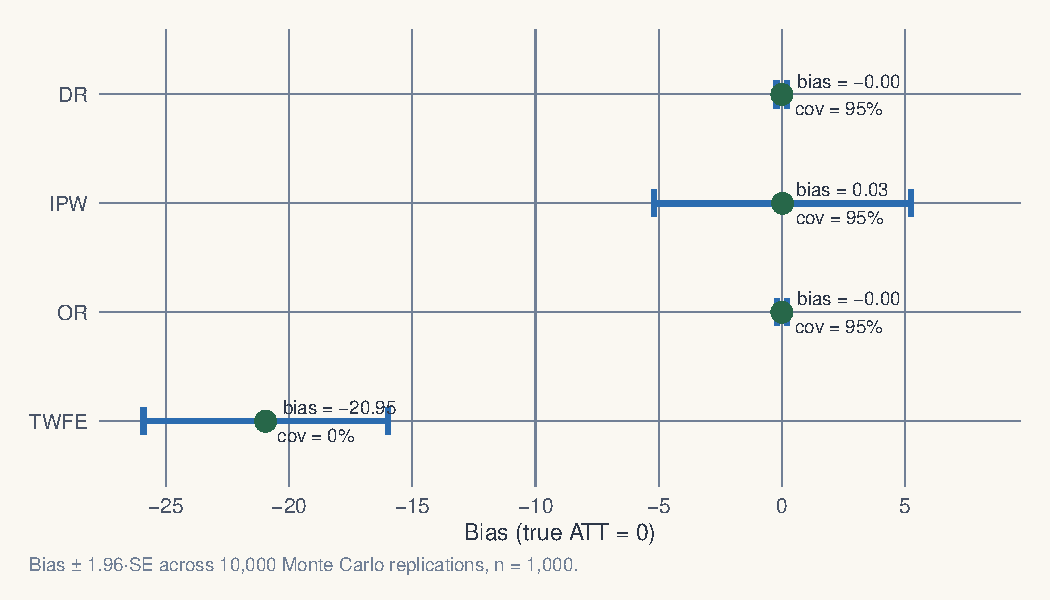
\includegraphics[width=0.68\textwidth]{figures/mc_dr_1.pdf}
\end{center}
\end{frame}

%% ----------
\begin{frame}{DGP 4: both models wrong}
\vspace{0.4em}
\begin{center}
\small\renewcommand{\arraystretch}{1.3}
\begin{tabular}{@{}lrrrrr@{}}
\toprule
      & \textbf{Bias} & \textbf{RMSE} & \textbf{SE} & \textbf{Coverage} & \textbf{CI length} \\
\midrule
TWFE  & $-16.38$ & $16.54$ & $3.63$ & $0.000$ & $14.22$ \\
OR    & $-5.20$  & $5.36$  & $1.29$ & $0.015$ & $5.05$  \\
\rowcolor{remixgreenlight}
IPW   & $-1.08$  & $2.66$  & $2.37$ & $0.949$ & $9.31$  \\
DR    & $-3.19$  & $3.45$  & $1.29$ & $0.308$ & $5.07$  \\
\bottomrule
\end{tabular}
\end{center}
\vspace{0.3em}
\begin{center}\small\color{warmgray}\itshape
DR undercovers at 0.31. IPW wins. Doubly robust $\neq$ doubly unbeatable.
\end{center}
\end{frame}

%% ----------
\begin{frame}{DGP 4: the sampling distribution}
\vspace{0.3em}
\begin{center}
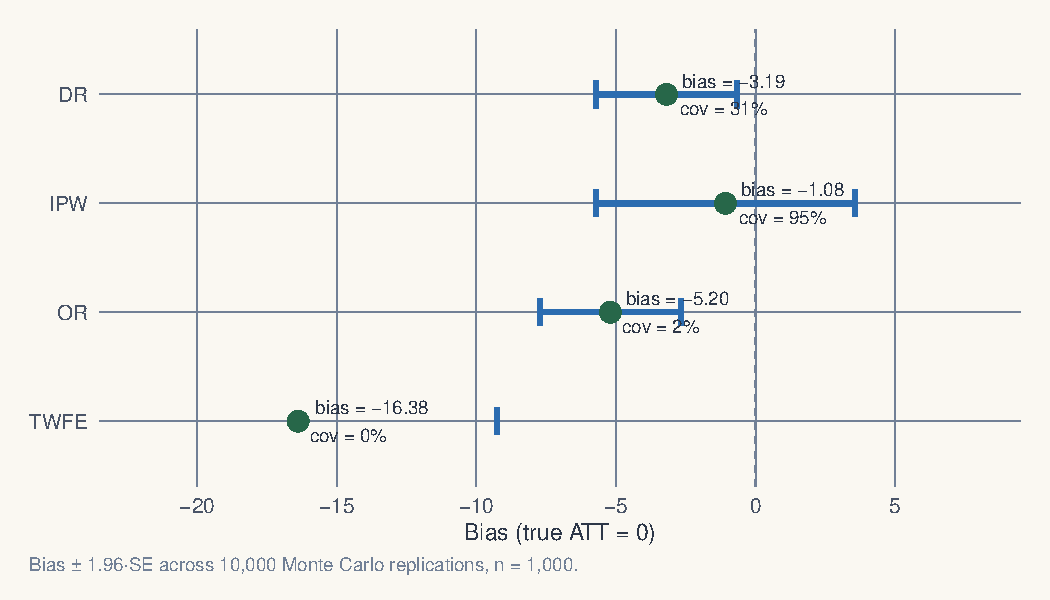
\includegraphics[width=0.68\textwidth]{figures/mc_dr_2.pdf}
\end{center}
\end{frame}

%% ----------
\begin{frame}{What the Monte Carlo teaches}
\vspace{0.8em}
\begin{itemize}\setlength\itemsep{0.55em}
  \item \textbf{TWFE + additive $X$:} coverage zero in every DGP. \highlight{Stop using it as a default.}
  \item \textbf{OR:} efficient when right. Coverage 1.5\% when wrong.
  \item \textbf{IPW:} less efficient, but robust to outcome misspecification.
  \item \textbf{DR:} best when one model is right. No better than IPW when both are wrong.
\end{itemize}
\end{frame}

%% ====================================================================
%% CONCLUSION
%% ====================================================================

\begin{frame}{Adding $X$ doesn't make your DiD credible}
\vspace{1.0em}
\begin{center}
\large
Adding $X$ shifts the credibility question---\\[0.6em]
from \highlight{``does PT hold?''}\\[0.5em]
to \highlight{``is my model of $Y(0)$ or $p(X)$ correct?''}\\[0.8em]
\color{warmgray}\normalsize
You still have to answer it.
\end{center}
\end{frame}

%% ====================================================================
%% PART 7 — LALONDE APPLICATION
%% ====================================================================

\begin{frame}{Now let's see it with real data}
\vspace{1.2em}
\begin{center}
\Large
LaLonde (1986) \textperiodcentered\ Dehejia \& Wahba (2002)
\end{center}
\vspace{0.8em}
\begin{center}
\color{warmgray}
A famous dataset where we \highlight{know the true effect.}\\[0.4em]
The benchmark: \highlight{\$1,794}.
\end{center}
\end{frame}

%% ----------
\begin{frame}{LaLonde (1986): the RCT found $\approx$\$800}
\vspace{0.8em}
\begin{itemize}\setlength\itemsep{0.6em}
  \item Job training program (National Supported Work Demonstration)
  \item Randomized --- treated and control groups assigned by lottery
  \item RCT estimate: earnings effect $\approx$ \textbf{\$800}
\end{itemize}
\vspace{0.6em}
\begin{center}\color{warmgray}\small
A clean causal estimate. The benchmark exists.
\end{center}
\end{frame}

%% ----------
\begin{frame}{LaLonde: dropped the RCT controls, used CPS instead}
\vspace{0.6em}
\begin{itemize}\setlength\itemsep{0.55em}
  \item Replaced the randomized controls with observational data (CPS, PSID)
  \item Re-ran every evaluator method from the literature
  \item Results ranged from \textbf{$-$\$16,000 to $+$\$3,000}
\end{itemize}
\vspace{0.5em}
\emphbox{The true effect was \$800. Not one method recovered it. \\
\textit{``The available evidence calls into serious question the ability of nonexperimental evaluators\ldots''}}
\vspace{0.3em}
\begin{center}\color{warmgray}\small
Empirical labor economics faces an evaluation problem.
\end{center}
\end{frame}

%% ----------
\begin{frame}{Dehejia \& Wahba (2002): propensity scores get close}
\vspace{0.6em}
\begin{itemize}\setlength\itemsep{0.55em}
  \item Need \textbf{two pre-treatment years} for all datasets --- uses a shorter sample
  \item RCT benchmark on this shorter sample: \highlight{\$1,794}
  \item Applied propensity score matching on the non-experimental sample
  \item Result: estimates close to \$1,794
\end{itemize}
\vspace{0.5em}
\begin{center}\color{warmgray}\small
Selective use of the data $+$ right method $=$ nearly recovered the truth.
\end{center}
\end{frame}

%% ----------
\begin{frame}{Our exercise: DiD with and without covariates}
\vspace{0.8em}
\begin{center}
NSW treated $+$ CPS controls \textperiodcentered\
Pre = 1975 \textperiodcentered\ Post = 1978\\[0.6em]
\large We know the effect: \highlight{\$1,794}\\[0.6em]
\normalsize\color{warmgray}
Let's see which specs recover it --- and which don't.
\end{center}
\end{frame}

%% ---------- Spec 0 ----------
\begin{frame}[fragile]{Naive TWFE: \$3,621 --- almost double the truth}
\vspace{0.4em}
\begin{lstlisting}[language=]
reg re i.post##i.ever_treated, robust
\end{lstlisting}
\vspace{0.5em}
\begin{center}
\begin{tabular}{lrr}
\toprule
Estimator & ATT & vs benchmark \\
\midrule
Naive TWFE & \textbf{\$3,621} & \textcolor{red}{$+$\$1,827} \\
\bottomrule
\end{tabular}
\end{center}
\vspace{0.4em}
\begin{center}\color{warmgray}\small
No covariates --- the CPS controls trend very differently from NSW treated.
\end{center}
\end{frame}

%% ---------- Spec A ----------
\begin{frame}[fragile]{Additive $X$: still \$3,621}
\vspace{0.4em}
\begin{lstlisting}[language=]
reg re i.post##i.ever_treated $X, robust
\end{lstlisting}
\vspace{0.5em}
\begin{center}
\begin{tabular}{lrr}
\toprule
Estimator & ATT & vs benchmark \\
\midrule
Additive $X$ & \textbf{\$3,621} & \textcolor{red}{$+$\$1,827} \\
\bottomrule
\end{tabular}
\end{center}
\vspace{0.4em}
\emphbox{Adding $X$ as time-invariant regressors does nothing here. The unit FE absorbs the level differences. The trend bias remains.}
\end{frame}

%% ---------- Spec B ----------
\begin{frame}[fragile]{Post$\,\times\,X$: \$1,711 --- now in the right range}
\vspace{0.4em}
\begin{lstlisting}[language=]
reg re i.post##i.ever_treated ///
    i.post##c.age i.post##c.agesq i.post##c.agecube ///
    i.post##c.educ i.post##c.educsq ///
    i.post##i.marr i.post##i.nodegree ///
    i.post##i.black i.post##i.hisp ///
    i.post##c.re74 i.post##i.u74, robust
\end{lstlisting}
\vspace{0.4em}
\begin{center}
\begin{tabular}{lrr}
\toprule
Estimator & ATT & vs benchmark \\
\midrule
Post$\,\times\,X$ & \textbf{\$1,711} & $-$\$83 \\
\bottomrule
\end{tabular}
\end{center}
\end{frame}

%% ---------- Spec C ----------
\begin{frame}[fragile]{Saturated TWFE: \$1,770}
\vspace{0.3em}
\begin{lstlisting}[language=]
* First-difference, then regress dy on X + D x X interactions
reg dy $X ///
    i.ever_treated#c.age i.ever_treated#c.agesq ///
    i.ever_treated#c.educ i.ever_treated#c.re74 ///
    i.ever_treated, robust
* Predict counterfactuals; ATT = mean(tau_sat) for treated
\end{lstlisting}
\vspace{0.3em}
\begin{center}
\begin{tabular}{lrr}
\toprule
Estimator & ATT & vs benchmark \\
\midrule
Saturated TWFE & \textbf{\$1,770} & $-$\$24 \\
\bottomrule
\end{tabular}
\end{center}
\end{frame}

%% ---------- OR ----------
\begin{frame}[fragile]{OR (HIT 1997): same answer as saturated TWFE}
\vspace{0.3em}
\begin{lstlisting}[language=]
* Fit trend model on controls only
reg dy $X if ever_treated == 0, robust
predict dy_hat
* ATT = mean gap for treated
gen delta_hat = dy - dy_hat if ever_treated == 1
\end{lstlisting}
\vspace{0.4em}
\begin{center}
\begin{tabular}{lrr}
\toprule
Estimator & ATT & vs benchmark \\
\midrule
OR by hand / \texttt{drdid reg} & \textbf{\$1,770} & $-$\$24 \\
\bottomrule
\end{tabular}
\end{center}
\vspace{0.2em}
\begin{center}\color{warmgray}\small
Saturated TWFE and OR are algebraically equivalent in the 2-period case.
\end{center}
\end{frame}

%% ---------- IPW ----------
\begin{frame}[fragile]{IPW (Abadie 2005): \$1,861}
\vspace{0.3em}
\begin{lstlisting}[language=]
drdid re $X, time(year) ivar(id) tr(ever_treated) ipw
\end{lstlisting}
\vspace{0.5em}
\begin{center}
\begin{tabular}{lrr}
\toprule
Estimator & ATT & vs benchmark \\
\midrule
IPW & \textbf{\$1,861} & $+$\$67 \\
\bottomrule
\end{tabular}
\end{center}
\end{frame}

%% ---------- DR ----------
\begin{frame}[fragile]{DR (Sant'Anna--Zhao 2020): \$1,979}
\vspace{0.3em}
\begin{lstlisting}[language=]
drdid re $X, time(year) ivar(id) tr(ever_treated) dripw
\end{lstlisting}
\vspace{0.5em}
\begin{center}
\begin{tabular}{lrr}
\toprule
Estimator & ATT & vs benchmark \\
\midrule
DR & \textbf{\$1,979} & $+$\$185 \\
\bottomrule
\end{tabular}
\end{center}
\end{frame}

%% ---------- Forest plot ----------
\begin{frame}{All seven estimators vs the \$1,794 benchmark}
\vspace{0.2em}
\begin{center}
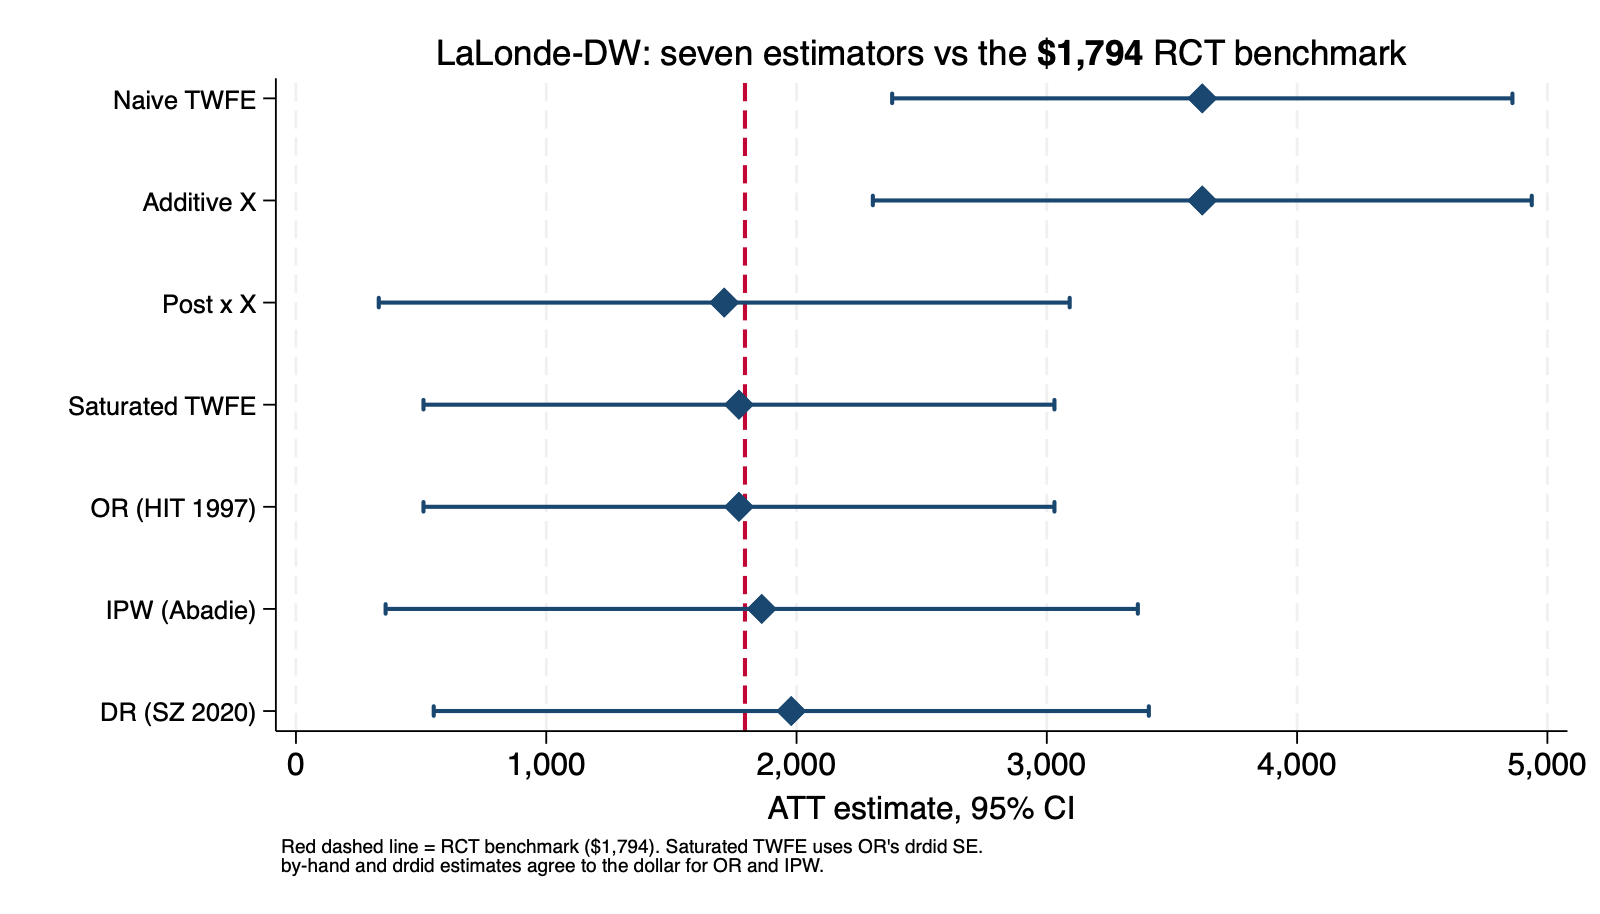
\includegraphics[width=0.82\textwidth]{figures/lalonde_forest.png}
\end{center}
\end{frame}

%% ---------- Conclusion ----------
\begin{frame}{Covariates are not robustness checks --- they are design}
\vspace{0.8em}
\begin{itemize}\setlength\itemsep{0.6em}
  \item People say: \textit{``if adding covariates changes results, be suspicious.''}
  \item That gets it backwards.
  \item We \highlight{know} the effect is \$1,794.
  \item Without covariates, or with additive covariates, we get \$3,621 --- \textit{wrong}.
  \item The correct specs recover \$1,770--\$1,979 --- \textit{right}.
\end{itemize}
\vspace{0.4em}
\emphbox{Covariates fix broken parallel trends. Changing your result is not a bug. It is the design working.}
\end{frame}

%% ---------- Closing linger ----------
\begin{frame}[plain]
\begin{tikzpicture}[remember picture,overlay]
\fill[cream] (current page.south west) rectangle (current page.north east);
\node[anchor=center, text width=0.84\paperwidth, align=center, text=charcoal]
  at (current page.center) {%
  \fontsize{18pt}{26pt}\selectfont
  The question is never\\[0.3em]
  {\color{accent}\bfseries ``did I control for $X$?''}\\[0.6em]
  The question is always\\[0.3em]
  {\color{accent}\bfseries ``did I get the model right?''}
};
\draw[accent, line width=1pt]
  ([yshift=1.4cm,xshift=0.25\paperwidth]current page.south west)
  -- ([yshift=1.4cm,xshift=-0.25\paperwidth]current page.south east);
\end{tikzpicture}
\end{frame}

\end{document}
